\section{Resoconto attività di verifica}
In questa sezione vengono descritti e analizzati gli esiti delle attività
di verifica svolte su tutti i documenti che vengono consegnati nelle varie 
revisioni di avanzamento del progetto.
\subsection{Revisioni}
\subsubsection{Revisione dei requisiti}
\paragraph{Tracciamento dei casi d'uso e dei requisiti}\mbox{}\\
Per facilitare il tracciamento delle relazioni fra casi d'uso e requisiti che
fra requisiti e fonti, il gruppo ha deciso di utilizzare il software PragmaDB.

\paragraph{Analisi statica dei documenti}\mbox{}\\
L'analisi dei documenti mediante \textit{Walkthrough}\glo{} ha portato 
all'individuazione di alcuni errori frequenti a partire dai quali è stata 
stilata una lista di controllo interna. In questo modo sarà possibile applicare
l'\textit{Inspection}\glo{} per le future attività di verifica.

\subsubsection{Revisione di progettazione}
\paragraph{Analisi statica del codice}\mbox{}\\
La stesura del codice è supportata dai plugin dell'editor Visual Studio Code. I plugin rilevanti in ambito di verifica sono due:
\begin{itemize}
	\item \textbf{ESLint v1.8.1}: linter per il linguaggio JavaScript;
	\item \textbf{Solidity v0.0.49}: linter per il linguaggio Solidity.
\end{itemize}
 I linter hanno aiutato notevolmente la stesura di codice sintatticamente corretto e alla standardizzazione del codice scritto, che risulta più uniforme; inoltre hanno facilitato parzialmente il processo di debugging.
 
\subsubsection{Revisione di qualifica}
\paragraph{Test}\mbox{}\\
Abbiamo preparato i test di accettazione e di sistema, i quali sono riportati nella Specifica dei test. Tali test verranno implementati per la revisione di accettazione.\\
%aggiungere label a sezione Specifica dei test
I test di integrazione e di unità sono in fase di costruzione.\\
Abbiamo creato e implementato test di unità sui contratti di backend per controllare la correttezza del codice e guidarne l'implementazione. 
Per la preparazione dei test sono serviti i seguenti strumenti:
\begin{itemize}
	\item \textbf{Truffle v5.0.4}: è usato il comando \texttt{truffle test};
\end{itemize}

\subsection{Esiti delle revisioni}
\subsubsection{Revisione dei Requisiti}
Successivamente alla prima revisione, il gruppo, basandosi sulle 
segnalazioni ricevute, ha apportato varie modifiche ai documenti. 
Di seguito vengono descritte brevemente tali modifiche:
\begin{itemize}
	\item in ogni documento è stato cambiato il nome della sezione 
	riportante le modifiche effettuate da "Tabella delle modifiche" a 
	"Registro delle modifiche";
	\item in ogni documento è stato inserito il numero di pagine totali 
	affianco al numero di pagina corrente;
	\item è stato cambiato il nome di alcune sezioni per renderle uniformi 
	con gli altri documenti;
	\item \textbf{Norme di Progetto} è stata aggiunta una sezione dove 
	vengono presentate le metriche relative ai processi. È stata aggiunta
	una sezione riguardante la formazione dei membri del gruppo;
	\item \textbf{Analisi dei Requisiti} seguendo le indicazioni del 
	professor Cardin sono state apportate modifiche ai casi d'uso e ai requisiti;
	\item \textbf{Piano di Progetto} è stata aggiunta una sezione per il 
	preventivo a finire. È stato spostato il focus dalla documentazione per concentrarsi di più sui processi e sulla loro applicazione secondo il modello incrementale;
	\item \textbf{Piano di Qualifica} le definizioni 
	delle metriche dei processi sono state spostate nelle \textit{Norme di Progetto}, mantenendo nel \textit{Piano di Qualifica} solamente le formule di calcolo, le soglie e gli intervalli.
\end{itemize}


\subsubsection{Revisione di Progettazione}
Successivamente alla seconda revisione, il gruppo, basandosi sulle 
segnalazioni ricevute, ha apportato varie modifiche ai documenti. 
Di seguito vengono descritte brevemente tali modifiche:
\begin{itemize}
	\item sono stati aggiornati i riferimenti nei documenti, inserendo dettagli relativi ai libri e alle collezioni secondo il sistema Vancouver (vedi \textit{Norme di Progetto v3.0.0}), specificando inoltre le parti di interesse;
	\item è stata aggiornata la forma di alcune espressioni al fine di evitare ridondanze;
	\item \textbf{Norme di Progetto} sono stati aggiornati i riferimenti del documento secondo le segnalazioni. \`E stata ristrutturata la sezione relativa alle attività del processo di fornitura ed è stata ampliata la sezione relativa al processo di sviluppo;
	\item \textbf{Analisi dei Requisiti} effettuati i cambiamenti in base alle segnalazioni al fine di correggere gli errori residui per rendere definitivo il documento;
	\item \textbf{Piano di Progetto} modificato consuntivo di periodo al fine di assolvere allo scopo dello stesso. Aggiornata la lista dei rischi avvenuti da inizio progetto;
	\item \textbf{Piano di Qualifica} ricondotta la specifica dei test alla qualità di prodotto. Spostata appendice attenente alle \textit{Norme di Progetto} e distribuita nelle sottosezioni adeguate. Ristrutturata appendice relativa all'attività di verifica.
\end{itemize}

\subsection{Calcolo delle metriche}
% DISCLAIMER: per ordinare le metriche, seguo l'ordine in cui sono definite qui nel PdQ
\subsubsection{Premessa relativa al periodo di progettazione e codifica della Technology Baseline}
Data la natura fortemente mutevole del Proof of Concept è stato deciso di non tenere traccia delle metriche di prodotto durante il suo sviluppo. Infatti, nella fase di progettazione di dettaglio e codifica il prodotto cambierà radicalmente, e non ci sarà una vera e propria continuità rispetto al PoC. \newline
Alcune delle metriche sulla pianificazione non erano calcolabili, in quanto non si può dire di aver effettivamente soddisfatto dei requisiti, dunque si è rinunciato ad utilizzarle.
Cionondimeno, poiché è necessario poter avere una visione dell'andamento del progetto nel tempo, si è deciso di tenere traccia di tutte le metriche a partire dalla fase di progettazione in dettaglio e codifica. Saranno considerate le serie storiche con una quantità maggiore di dati a disposizione.
\subsubsection{Premessa relativa al periodo di progettazione di dettaglio e codifica}
Come visibile dai grafici, solamente una parte delle metriche è stata implementata. Questo è dovuto ad alcune difficoltà nel loro reperimento.
Prevediamo un ampliamento durante il periodo di validazione e collaudo che, tardivo, avrà minore impatto sul prodotto, ma sarà utile a livello esperienziale ed educativo.\\
Le metriche di code coverage non soddisfano le soglie di accettabilità. Questo è dovuto a cambiamenti nell'implementazione del prodotto e conseguente ritardo nel testing dello stesso.

\subsubsection{Legenda}
Legenda per le abbreviazioni presenti in grafici e tabelle:
\begin{itemize}
	\item \textbf{-}: campi vuoti;
	\item \textbf{N}: nome del documento;
	\item \textbf{RR}: periodo di revisione dei requisiti;
	\item \textbf{C}: periodo di consolidamento dei requisiti;
	\item \textbf{TB}: periodo di progettazione e codifica della Technology Baseline;
	\item \textbf{PD}: periodo di progettazione di dettaglio e codifica;
	\item \textbf{VC}: periodo di validazione e collaudo.
\end{itemize}

\subsubsection{PROS - Percentuale di Requisiti Obbligatori Sodisfatti}
% PB In questo calcolo si tiene traccia dei requisiti associati ai test di sistema, tramite i test di sistema superati.
% 16/38
\begin{longtable}
	{ >{\centering}p{0.15\textwidth}
		>{\centering}p{0.15\textwidth} >{\centering}p{0.15\textwidth} >{\centering}p{0.15\textwidth} >{\centering}p{0.15\textwidth}}
	%\hline
	\rowcolor{white}\caption{PROS}\\
	\rowcolorhead
	\textbf{\color{white}RR} 
	& \textbf{\color{white}C} 
	& \textbf{\color{white}TB}
	& \textbf{\color{white}PD}
	& \textbf{\color{white}VC}
	\tabularnewline %\hline  
	\endhead
	
	0
	& 0\%
	& 0\%
	& 42\%
	& -
	\tabularnewline %\hline 
\end{longtable}

\subsubsection{EAC - Estimated At Completion}
\begin{figure}[H]
	\centering
	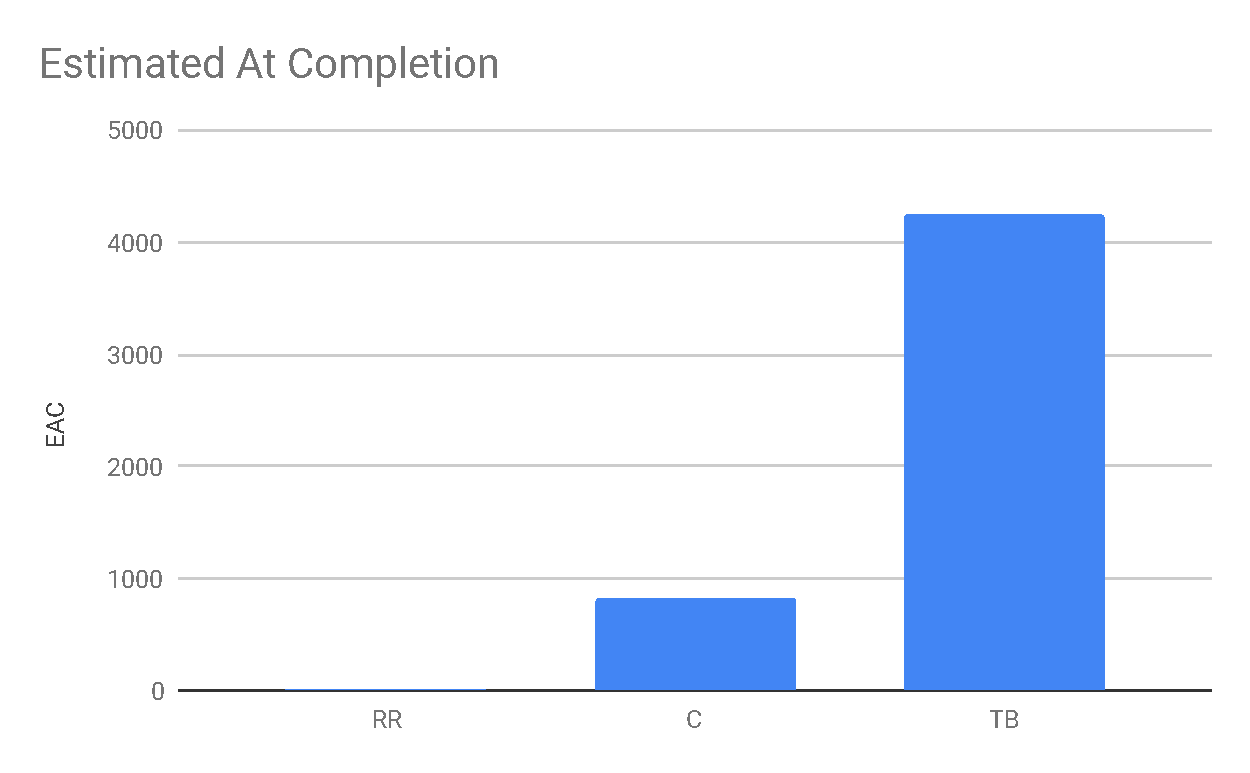
\includegraphics[scale=0.4]{res/images/eac.pdf}
	\caption{Estimated At Completion durante i periodi da RR a TB}
\end{figure}

%\subsubsection{Profondità della gerarchia}


\subsubsection{VAC - Variance At Completion}

\begin{figure}[H]
	\centering
	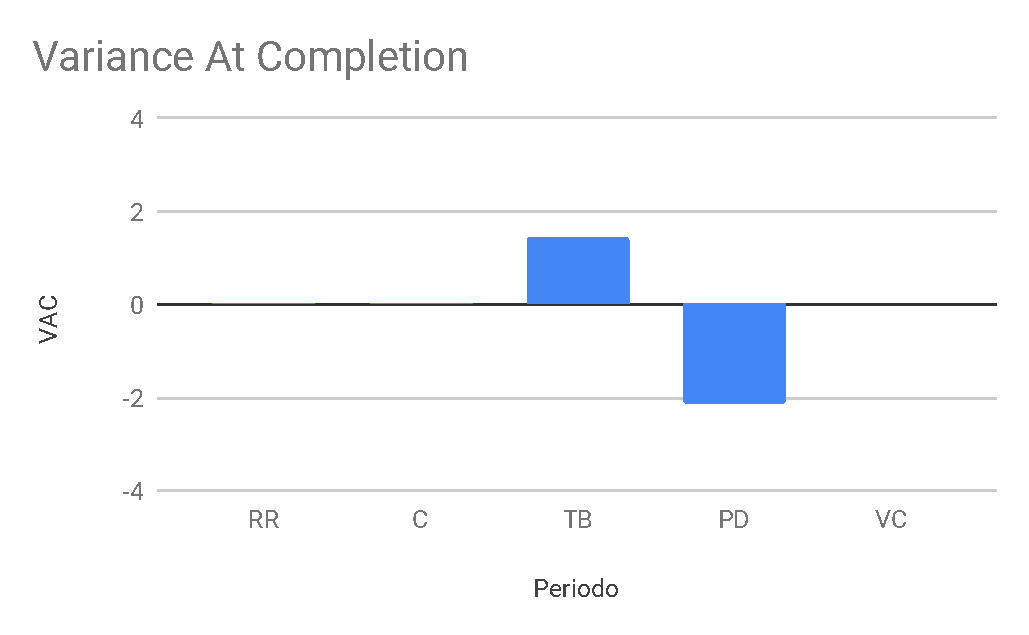
\includegraphics[scale=0.8]{res/images/RQ/vac.pdf}
	\caption{Variance At Completion}
\end{figure}
\pagebreak

\subsubsection{AC - Actual Cost}

\begin{figure}[H]
	\centering
	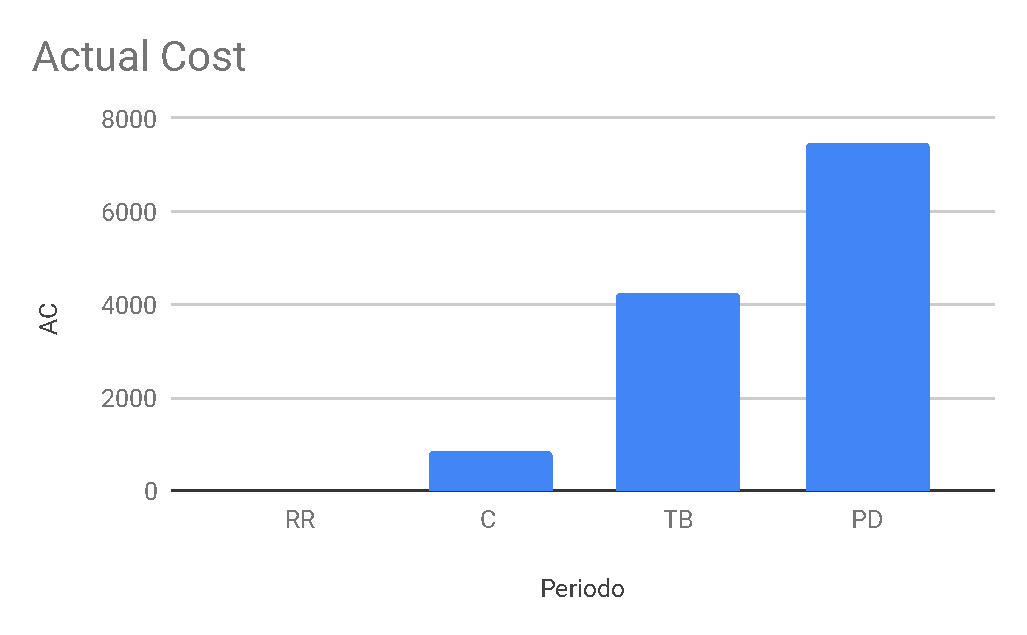
\includegraphics[scale=0.8]{res/images/RQ/ac.pdf}
	\caption{Actual Cost}
\end{figure}

\subsubsection{EV - Earned Value}

\begin{figure}[H]
	\centering
	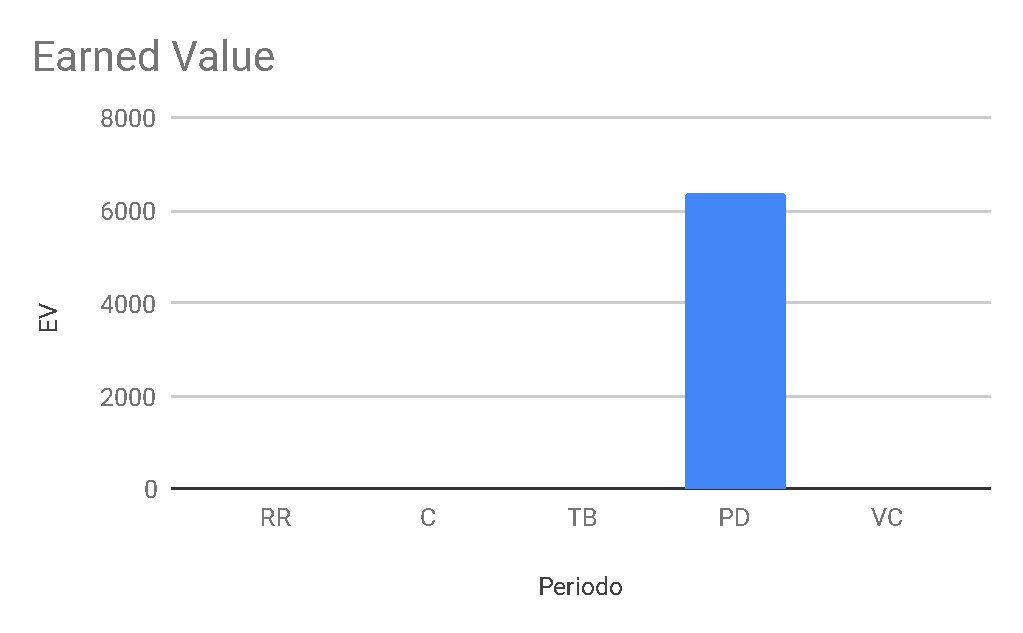
\includegraphics[scale=0.8]{res/images/RQ/ev.pdf}
	\caption{Earned Value}
\end{figure}

\subsubsection{PV - Planned Value}

\begin{figure}[H]
	\centering
	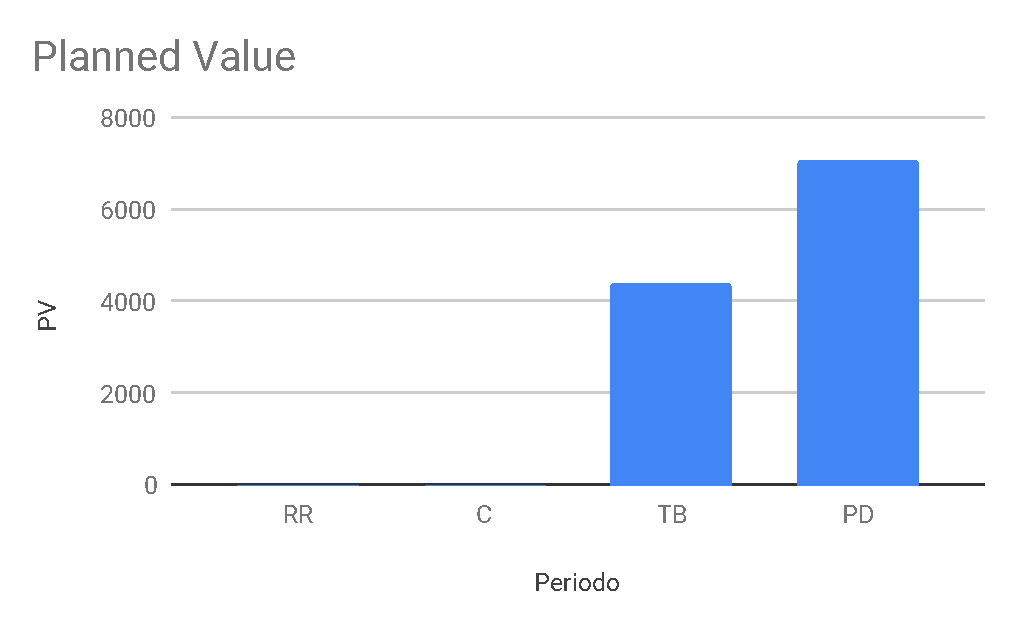
\includegraphics[scale=0.8]{res/images/RQ/pv.pdf}
	\caption{Planned Value}
\end{figure}

\subsubsection{SV - Schedule Variance}

\begin{figure}[H]
	\centering
	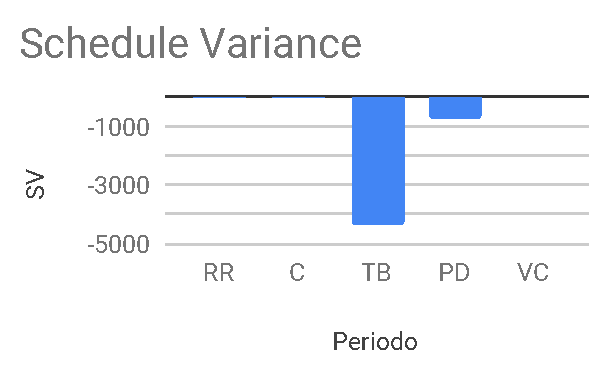
\includegraphics[scale=0.8]{res/images/RQ/sv.pdf}
	\caption{Schedule Variance}
\end{figure}

\subsubsection{CV - Cost Variance}
\begin{figure}[H]
	\centering
	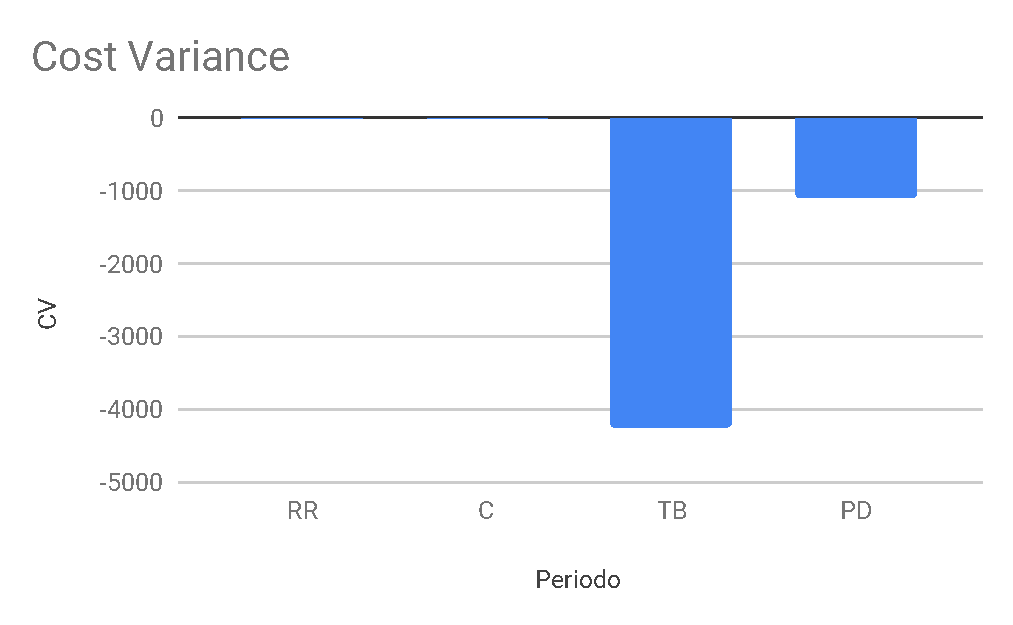
\includegraphics[scale=0.8]{res/images/RQ/cv.pdf}
	\caption{Schedule Variance}
\end{figure}


\subsubsection{Code Coverage}
\paragraph{Statement coverage}\mbox{}\\
\begin{figure}[H]
	\centering
	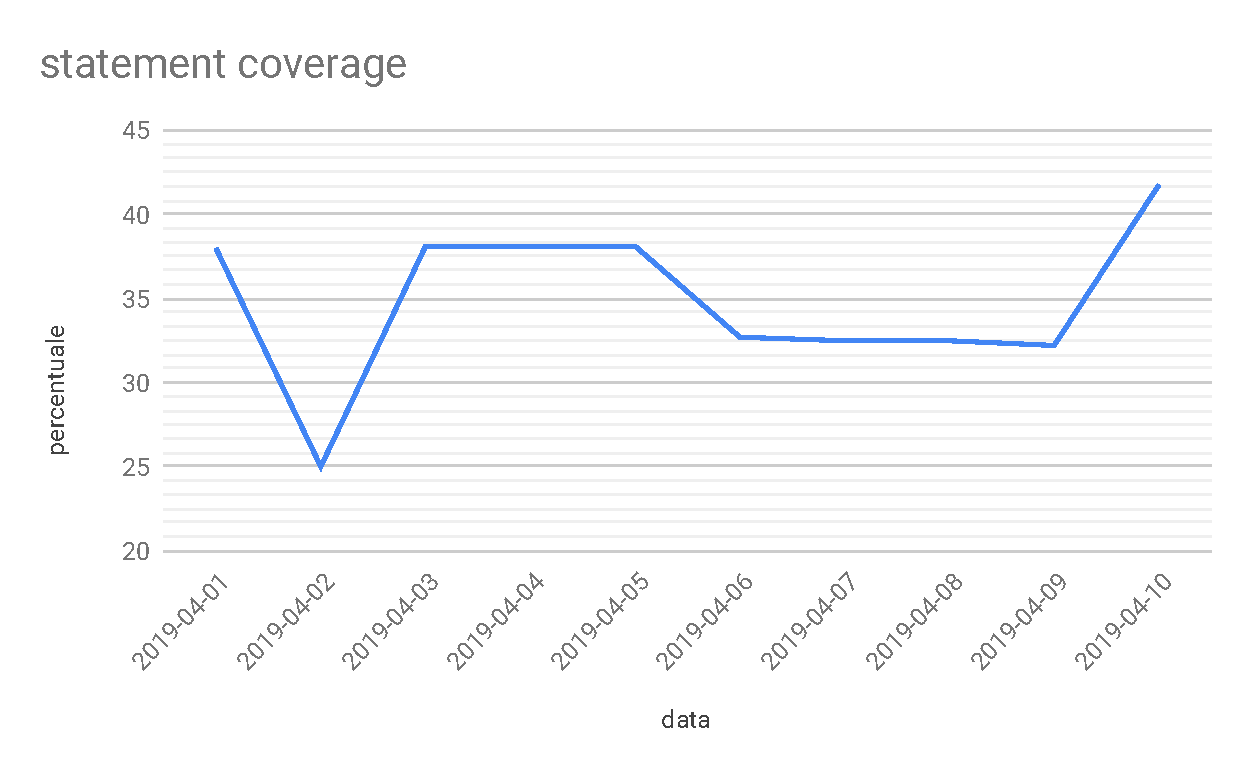
\includegraphics[scale=0.6]{res/images/RQ/statement-coverage-RQ.pdf}
	\caption{Statement coverage}
\end{figure}	
\paragraph{Branch coverage}\mbox{}\\
\begin{figure}[H]
	\centering
	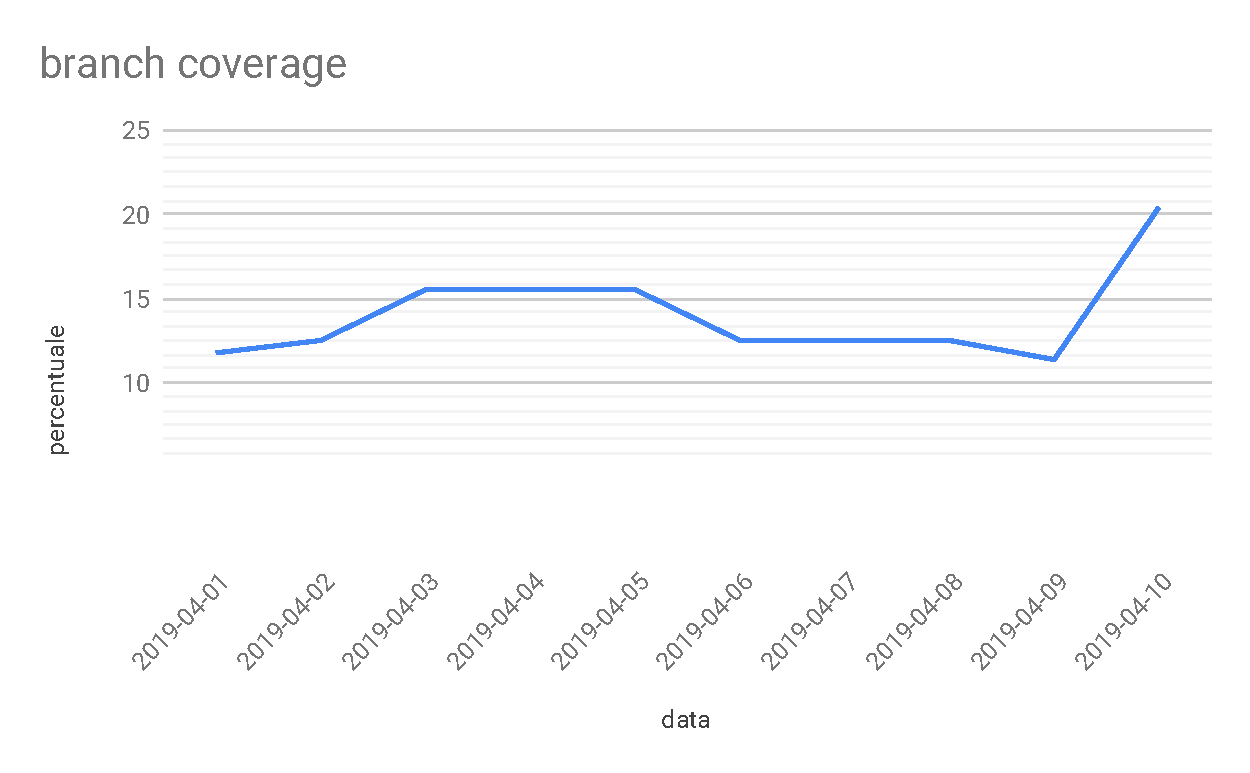
\includegraphics[scale=0.6]{res/images/RQ/branch-coverage-RQ.pdf}
	\caption{Branch coverage}
\end{figure}
\paragraph{Function coverage}\mbox{}\\
\begin{figure}[H]
	\centering
	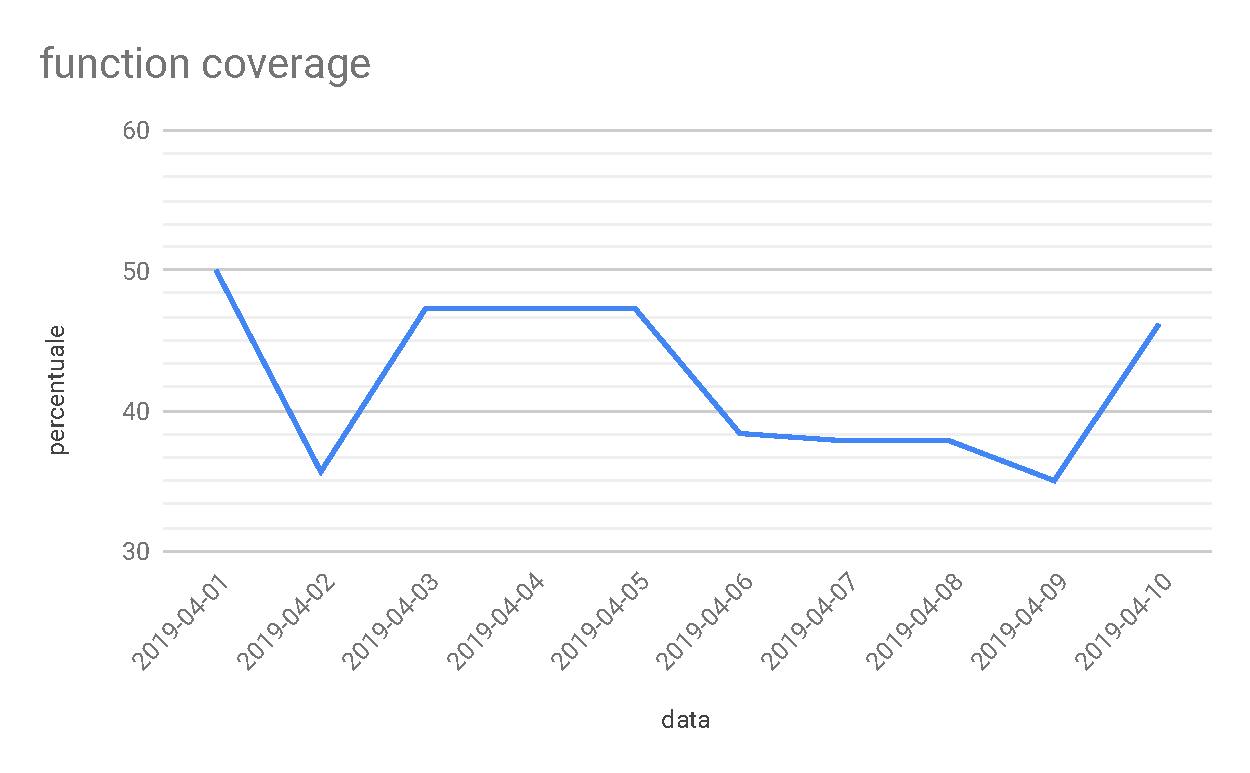
\includegraphics[scale=0.6]{res/images/RQ/function-coverage-RQ.pdf}
	\caption{Function coverage}
\end{figure}
\paragraph{Line coverage}\mbox{}\\
\begin{figure}[H]
	\centering
	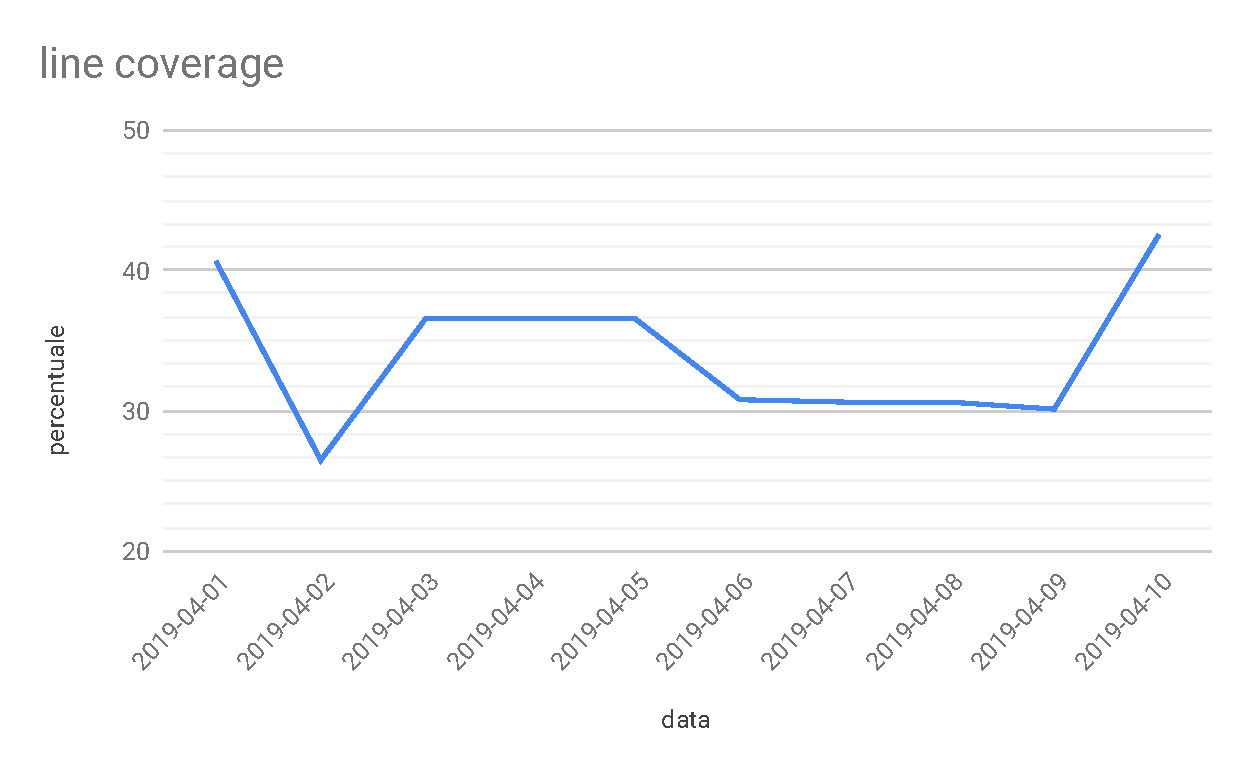
\includegraphics[scale=0.6]{res/images/RQ/line-coverage-RQ.pdf}
	\caption{Line coverage}
\end{figure}

\subsubsection{Facilità di utilizzo}

\subsubsection{Facilità di comprensione} % == CCR
\begin{figure}[H]
	\centering
	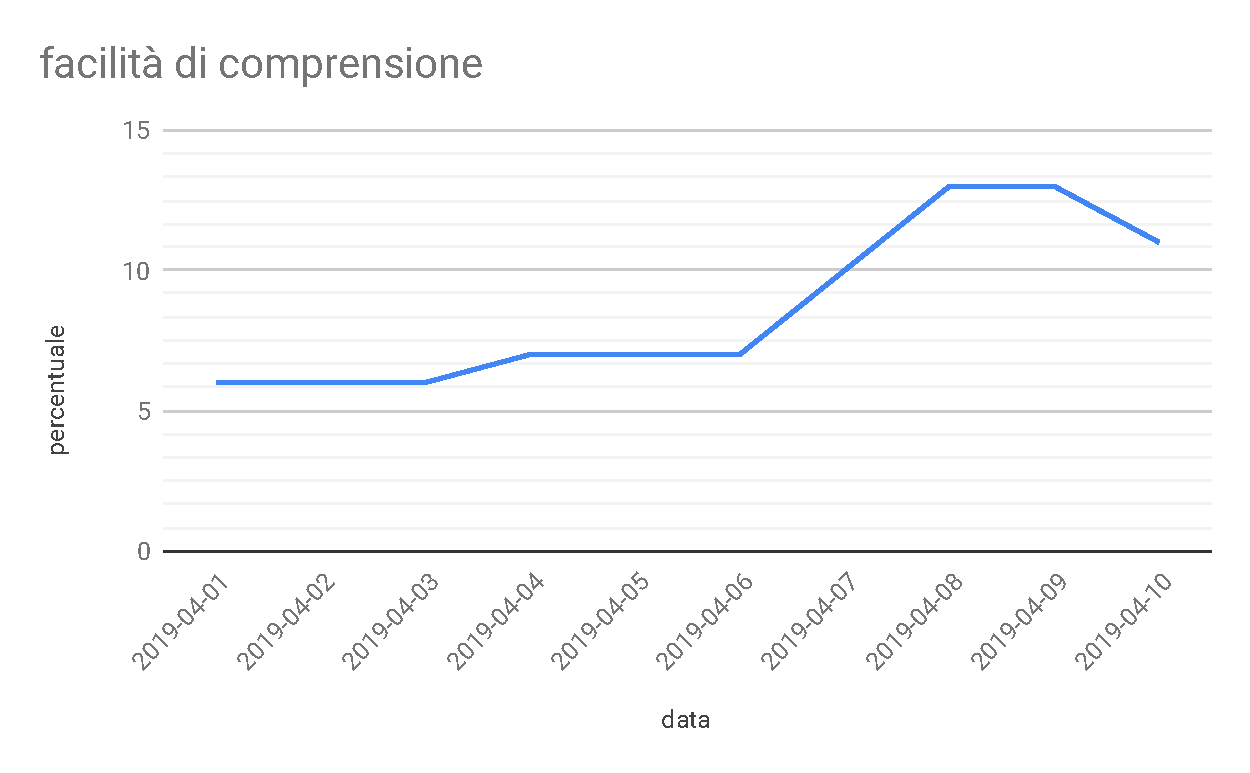
\includegraphics[scale=0.6]{res/images/RQ/facilita-di-comprensione.pdf}
	\caption{Facilità di comprensione}
\end{figure}

\pagebreak
\subsubsection{Indice di Gulpease}

\begin{longtable}{ >{\centering}p{0.15\textwidth} >{\centering}p{0.10\textwidth}	>{\centering}p{0.1075\textwidth} >{\centering}p{0.10\textwidth} >{\centering}p{0.10\textwidth} >{\centering}p{0.10\textwidth}}
	
	%\hline
	\rowcolor{white}\caption{Indice di Gulpease raggruppato per documento, lungo i periodi da RR a TB}\\
	\rowcolorhead
	\textbf{\color{white}N} 
	& \textbf{\color{white}RR} 
	& \centering\textbf{\color{white}C}
	& \textbf{\color{white}TB}
	& \textbf{\color{white}PD}
	& \textbf{\color{white}VC} 
	\tabularnewline %\hline 	
	
	\textit{Analisi dei requisiti}
	& 67
	& 66
	& 63
	& 63
	& -
	\tabularnewline %\hline 
	
	\textit{Glossario}
	& 71
	& 71
	& 71
	& 71
	& -
	\tabularnewline %\hline 
	
	\textit{Norme di progetto}
	& 65
	& 65
	& 63
	& 66
	& -
	\tabularnewline %\hline 
	
	\textit{Piano di progetto}
	& 68
	& 68
	& 66
	& 67
	& -
	\tabularnewline %\hline 
	
	\textit{Piano di qualifica}
	& 70
	& 70
	& 67
	& 65
	& -
	\tabularnewline %\hline 
	
	\textit{Studio di Fattibilità}
	& 73
	& -
	& -
	& -
	& -
	\tabularnewline %\hline 
	
	\textit{Verbali esterni (media)}
	& 72
	& 72
	& 66
	& 69
	& -
	\tabularnewline %\hline 
	
	\textit{Verbali interni (media)}
	& 74
	& 74
	& 70
	& 73
	& -
\end{longtable}
\begin{figure}[H]
	\centering
	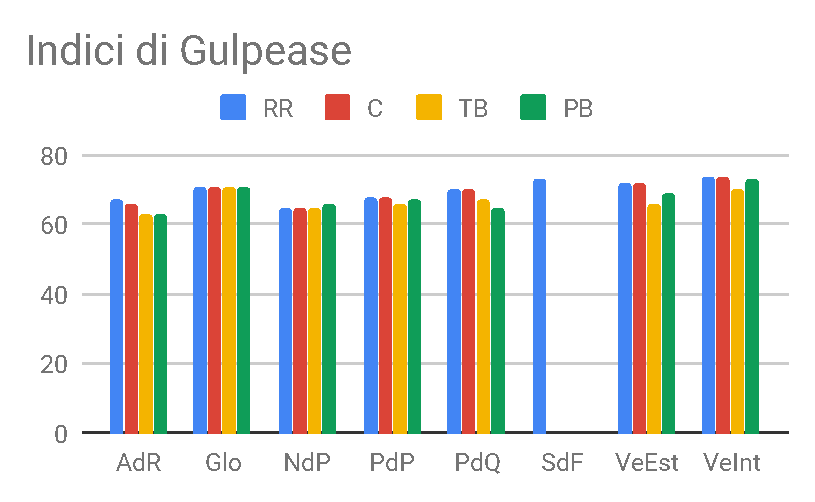
\includegraphics[scale=0.8]{res/images/RQ/gulpease.pdf}
	\caption{Indice di Gulpease}
\end{figure}



%\subsubsection{Semplicità delle classi}

\subsubsection{SLOC}

\begin{figure}[H]
	\centering
	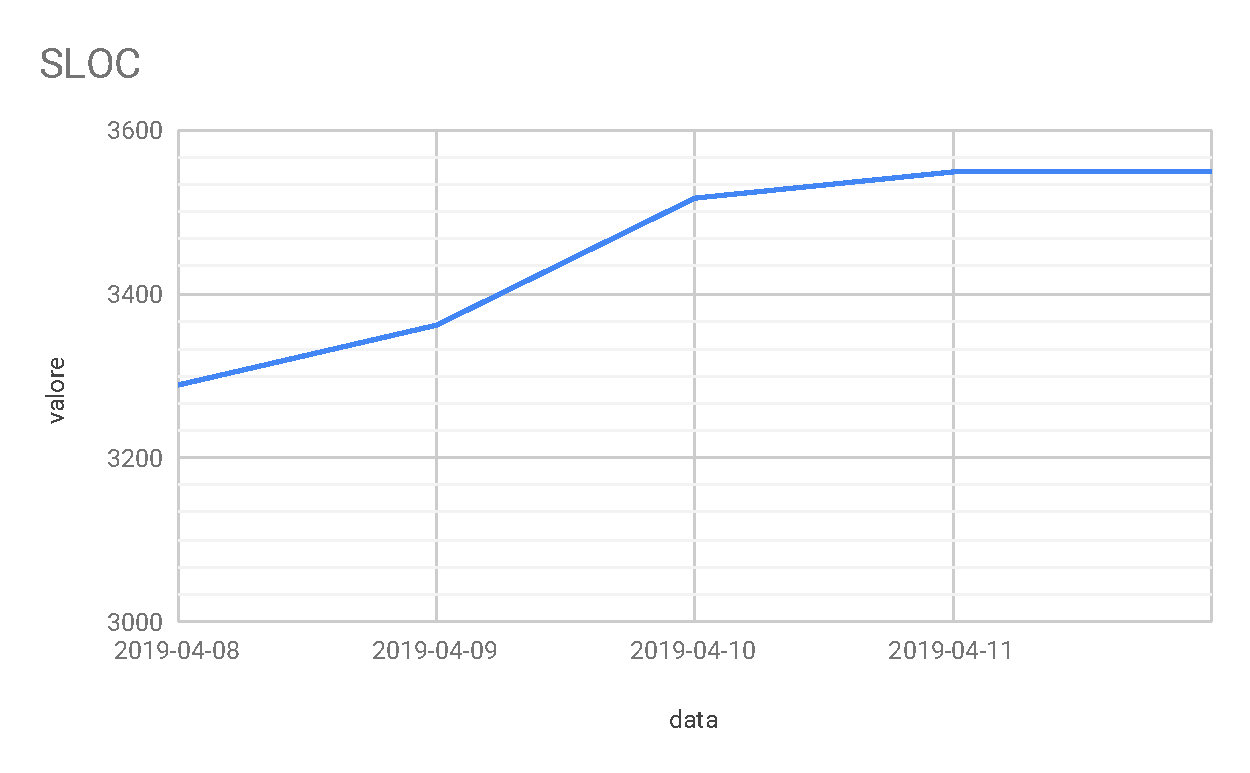
\includegraphics[scale=0.6]{res/images/RQ/sloc.pdf}
	\caption{Source lines of code}
\end{figure}



